% ME 3001 - Tristan Hill - Spring 2017
% Homework 7

% The 1D Heat Equation
% Solved With Finite Difference

% Document settings
\documentclass[11pt]{article}
\usepackage[margin=1in]{geometry}
\usepackage[pdftex]{graphicx}
\usepackage{multirow}
\usepackage{setspace}
\usepackage{hyperref}
\usepackage{color,soul}
\usepackage{fancyvrb}
\usepackage{framed}
\usepackage{wasysym}
\usepackage{amssymb}

\pagestyle{plain}
\setlength\parindent{0pt}
\hypersetup{
    bookmarks=true,         % show bookmarks bar?
    unicode=false,          % non-Latin characters in Acrobat’s bookmarks
    pdftoolbar=true,        % show Acrobat’s toolbar?
    pdfmenubar=true,        % show Acrobat’s menu?
    pdffitwindow=false,     % window fit to page when opened
    pdfstartview={FitH},    % fits the width of the page to the window
    pdftitle={My title},    % title
    pdfauthor={Author},     % author
    pdfsubject={Subject},   % subject of the document
    pdfcreator={Creator},   % creator of the document
    pdfproducer={Producer}, % producer of the document
    pdfkeywords={keyword1} {key2} {key3}, % list of keywords
    pdfnewwindow=true,      % links in new window
    colorlinks=true,       % false: boxed links; true: colored links
    linkcolor=red,          % color of internal links (change box color with linkbordercolor)
    citecolor=green,        % color of links to bibliography
    filecolor=magenta,      % color of file links
    urlcolor=blue           % color of external links
}

% assignment number 
\newcommand{\NUM}{6} 

\definecolor{mygray}{rgb}{.6, .6, .6}

\setulcolor{red} 
\setstcolor{green} 
\sethlcolor{mygray} 

\begin{document}

	\textbf{\LARGE ME 3001-001, Fall 2019} \\\\
	\textbf{\LARGE Activity : FDM - 1D Steady State Conduction } \\\\

		

		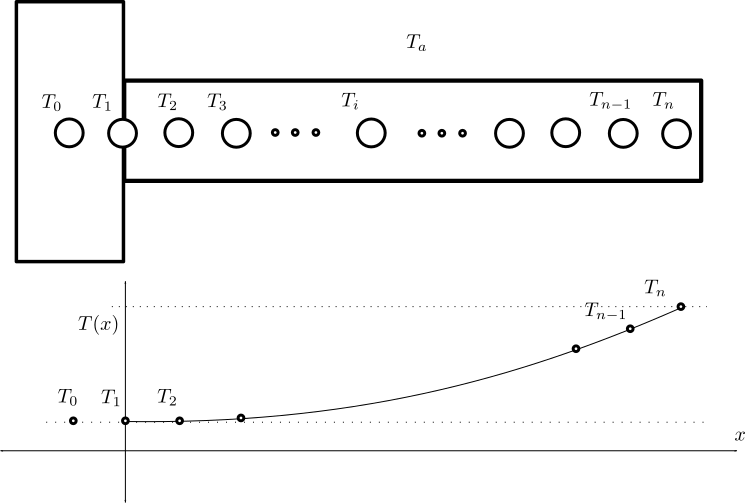
\includegraphics[scale=.5]{hw7_fig1.png}\\

		The {\it 1D Rod} undergoing conduction and convection can be modeled with following ODE. \\\\
\scalebox{1.5}{$\frac{d^2T}{dx^2}+h^*(T_a-T)=0$} \\\\
with boundary conditions: \scalebox{1}{$\hspace{5mm}T(x=L)=T_n,\hspace{5mm} \frac{dT}{dx}|_{x=0}=0$}\\\\
and constants:  \scalebox{1}{$h^*=0.05\hspace{2mm}(m^-2), \hspace{3mm}L=10\hspace{2mm}(m),\hspace{3mm}\Delta x=0.1\hspace{2mm}(m),\hspace{3mm}T_a=200\hspace{2mm}(K)$}
 
		
\end{document}



